\maketitle{}
\section{ Barrel File }

\subsection{ What is a Barrel File? }

A barrel File is a way to rollup exports from several modules into a signle
convenience module. The barrel itself is a module file that re-exports selected
exports of other modules.
\\
\\
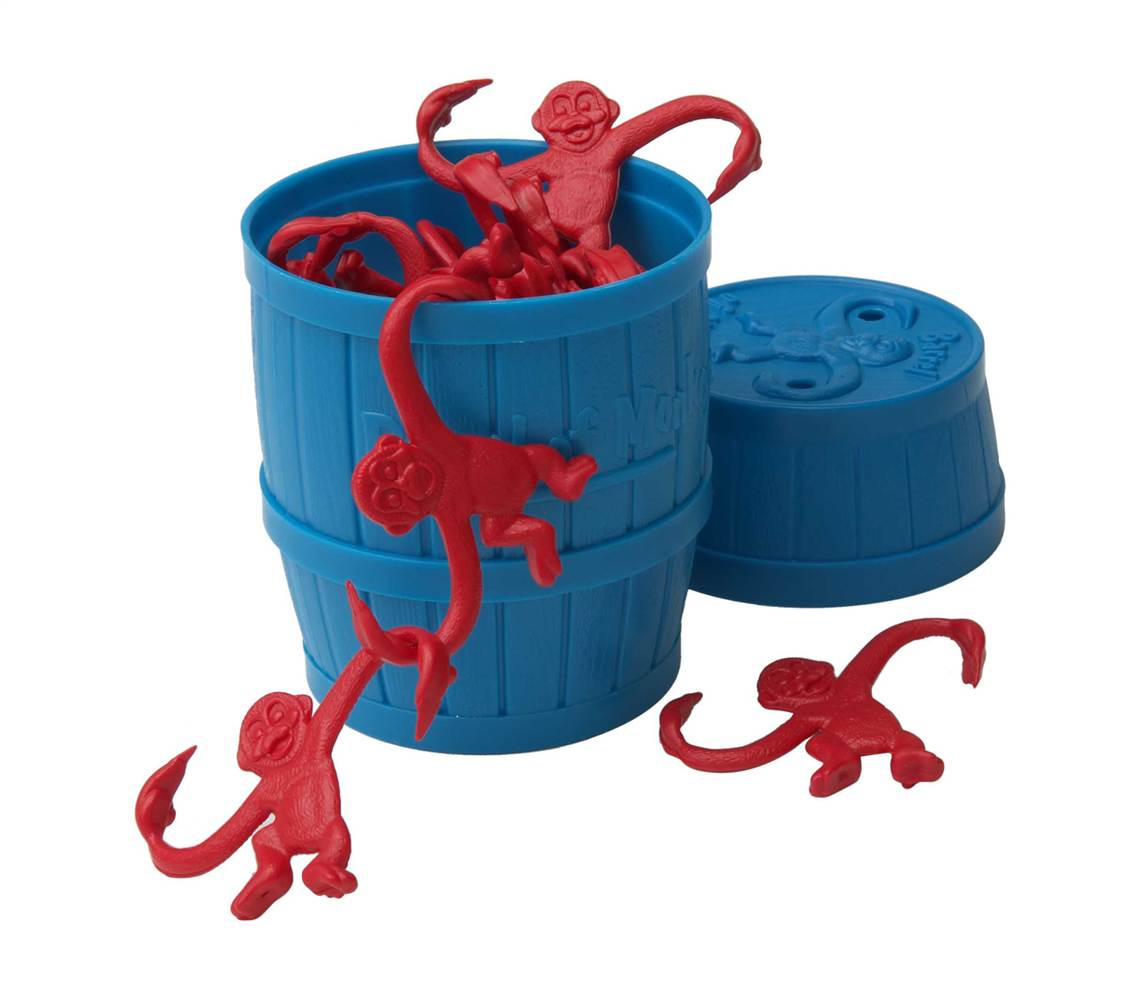
\includegraphics[width=12.1cm, height=9cm]{typescript/barrel-file/monkey-barrel}

\subsection{ Barrel File In Practice }
In the previous chapter we discussed doing something like the following:
\begin{lstlisting}
import {module} from '@ill/color-picker';
\end{lstlisting}

We are able to do this, because the nrwl nx layer on top Angular CLI, will
generate an index.tx file which will contain all imports. Anything that is
within the component, that should be exposed outside the lib, should be put
in the index.ts(barrel file).

\begin{lstlisting}
// index.ts
export { IllColorPickerModule } from './src/ill-color-picker.module';
\end{lstlisting}

\subsection{ Enforcing Barrel File With Tslint }
In addition, Nrwl nx has a tslint add on called nx-enforce-module-bounderies.
\begin{lstlisting}
// tslint.json
"nx-enforce-module-boundaries": [
      true,
      {
        "allow": [],
        "depConstraints": [
          {
            "sourceTag": "*",
            "onlyDependOnLibsWithTags": [
              "*"
            ]
          }
        ]
      }
    ],
\end{lstlisting}

Adding true, will make the tslint complain whenever we are not using the barrel
import when accesing a lib file.
